\chapter{A semiclassical approach to SHE}

\label{chapter3}

In this chapter, we shall look at the semi-classical picture of SHE and try to understand the mechanisms behind the phenomena.

\section{SHE revisited: relation with AHE}

As seen in \cref{sec:ohe}, the OHE results in a charge imbalance along the edges of the conductor in the presence of an external magnetic field. We have also seen that in the case of SHE (sec \ref{sec:she}), instead of a charge imbalance, we see a spin imbalance i.e. a preferential accumulation along the edges of the material.

Both AHE and SHE are similar in the way that there is a spin imbalance and hence an accumulation of carriers with opposite spins on opposite edges of the sample.
The only difference is that in the case of AHE, there is a net magnetization of the material (since we typically use magnetic materials for AHE).
This gives preferential scattering of the carriers based on spin but with unequal proportion i.e. due to the net magnetization of the material, the proportion of spin up \( \uparrow \) and spin down \( \downarrow \) is unequal and hence there will be disproportionate accumulation of one spin ($ \uparrow $ or $ \downarrow $) from another ($ \downarrow $ or $ \uparrow $).

A significant advantage of SHE over AHE is that the former doesn't require an external magnetic field to function.
As long as the material in question possesses a high spin-orbit interaction, SHE is observed and the conversion of pure charge current (unpolarized electrons) gets converted into pure spin current (polarized electrons) with no charge current \cite{hirsch1999spin}.

\subsection{Spin Hall angle (SHA)}

\label{subsec:spin-angle}

A parameter of importance in the context of SHE, is the spin Hall angle \( \theta_{SH} \) which is defined as

\begin{equation} \label{eq:sha}
    \theta_{SH} = \frac{\sigma^s_{xy} \: e}{\sigma^c_{xx} \: \hbar}
\end{equation}

where \( \sigma^s_{xy} \) is the transverse conductivity due to spin current, \( \sigma^c_{xx} \) is the longitudinal conductivity due to charge current, and \( e \) is the charge of an electron.

\( \theta_{SH} \) is the ratio of spin Hall conductivity to charge conductivity and quantifies the efficiency of conversion from charge to spin current and vice-versa.

\subsection{Spin Orbit interaction}

% TODO: Write section on spin orbit coupling


\section{Mechanisms behind the phenomena}

\label{sec:mechanisms}

Over the past century, the scientific community has agreed upon three plausible mechanisms responsible for SHE. These are categorized into extrinsic and intrinsic mechanisms. Let's dive into the details of the same.

\begin{figure}[h!]
    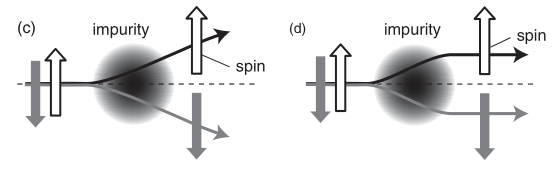
\includegraphics[width=\columnwidth]{she-mechanisms.png}
    \caption{Extrinsic scattering mechanisms responsible for SHE: (c) skew-scattering and (d) side jump\\ \vspace{0.2cm} \textit{Image credit: \cite{murakami2015spin}}}
\end{figure}


\subsection{Extrinsic: Skew-scattering}

\subsection{Extrinsic: Side-jump}

\subsection{Intrinsic}
